% Options for packages loaded elsewhere
\PassOptionsToPackage{unicode}{hyperref}
\PassOptionsToPackage{hyphens}{url}
%
\documentclass[
]{article}
\usepackage{amsmath,amssymb}
\usepackage{lmodern}
\usepackage{iftex}
\ifPDFTeX
  \usepackage[T1]{fontenc}
  \usepackage[utf8]{inputenc}
  \usepackage{textcomp} % provide euro and other symbols
\else % if luatex or xetex
  \usepackage{unicode-math}
  \defaultfontfeatures{Scale=MatchLowercase}
  \defaultfontfeatures[\rmfamily]{Ligatures=TeX,Scale=1}
\fi
% Use upquote if available, for straight quotes in verbatim environments
\IfFileExists{upquote.sty}{\usepackage{upquote}}{}
\IfFileExists{microtype.sty}{% use microtype if available
  \usepackage[]{microtype}
  \UseMicrotypeSet[protrusion]{basicmath} % disable protrusion for tt fonts
}{}
\makeatletter
\@ifundefined{KOMAClassName}{% if non-KOMA class
  \IfFileExists{parskip.sty}{%
    \usepackage{parskip}
  }{% else
    \setlength{\parindent}{0pt}
    \setlength{\parskip}{6pt plus 2pt minus 1pt}}
}{% if KOMA class
  \KOMAoptions{parskip=half}}
\makeatother
\usepackage{xcolor}
\IfFileExists{xurl.sty}{\usepackage{xurl}}{} % add URL line breaks if available
\IfFileExists{bookmark.sty}{\usepackage{bookmark}}{\usepackage{hyperref}}
\hypersetup{
  pdftitle={Butterfly scan},
  hidelinks,
  pdfcreator={LaTeX via pandoc}}
\urlstyle{same} % disable monospaced font for URLs
\usepackage[margin=1in]{geometry}
\usepackage{graphicx}
\makeatletter
\def\maxwidth{\ifdim\Gin@nat@width>\linewidth\linewidth\else\Gin@nat@width\fi}
\def\maxheight{\ifdim\Gin@nat@height>\textheight\textheight\else\Gin@nat@height\fi}
\makeatother
% Scale images if necessary, so that they will not overflow the page
% margins by default, and it is still possible to overwrite the defaults
% using explicit options in \includegraphics[width, height, ...]{}
\setkeys{Gin}{width=\maxwidth,height=\maxheight,keepaspectratio}
% Set default figure placement to htbp
\makeatletter
\def\fps@figure{htbp}
\makeatother
\setlength{\emergencystretch}{3em} % prevent overfull lines
\providecommand{\tightlist}{%
  \setlength{\itemsep}{0pt}\setlength{\parskip}{0pt}}
\setcounter{secnumdepth}{-\maxdimen} % remove section numbering
\newlength{\cslhangindent}
\setlength{\cslhangindent}{1.5em}
\newlength{\csllabelwidth}
\setlength{\csllabelwidth}{3em}
\newlength{\cslentryspacingunit} % times entry-spacing
\setlength{\cslentryspacingunit}{\parskip}
\newenvironment{CSLReferences}[2] % #1 hanging-ident, #2 entry spacing
 {% don't indent paragraphs
  \setlength{\parindent}{0pt}
  % turn on hanging indent if param 1 is 1
  \ifodd #1
  \let\oldpar\par
  \def\par{\hangindent=\cslhangindent\oldpar}
  \fi
  % set entry spacing
  \setlength{\parskip}{#2\cslentryspacingunit}
 }%
 {}
\usepackage{calc}
\newcommand{\CSLBlock}[1]{#1\hfill\break}
\newcommand{\CSLLeftMargin}[1]{\parbox[t]{\csllabelwidth}{#1}}
\newcommand{\CSLRightInline}[1]{\parbox[t]{\linewidth - \csllabelwidth}{#1}\break}
\newcommand{\CSLIndent}[1]{\hspace{\cslhangindent}#1}
\usepackage{float}
\let\origfigure\figure
\let\endorigfigure\endfigure
\renewenvironment{figure}[1][2] {
    \expandafter\origfigure\expandafter[H]
} {
    \endorigfigure
}
\ifLuaTeX
  \usepackage{selnolig}  % disable illegal ligatures
\fi

\title{Butterfly scan}
\author{}
\date{\vspace{-2.5em}}

\begin{document}
\maketitle

The algorithms and programs described here are in the repository on
GitHub:

\url{https://github.com/andy-aa/butterfly_scan}

The algorithms are implemented in the R programming
language{[}\protect\hyperlink{ref-R-base}{1}{]}.

\hypertarget{calculation-of-the-body-volume-of-a-butterfly}{%
\subsection{Calculation of the body volume of a
butterfly}\label{calculation-of-the-body-volume-of-a-butterfly}}

The algorithm for estimating the volume of the body of a butterfly:

\begin{enumerate}
\def\labelenumi{\arabic{enumi}.}
\tightlist
\item
  Converting a color image to black and white. Three-channel RGB image →
  Single-channel grayscale image → Single-channel black and white
  images. When converting an image to black and white, it is necessary
  to use an empirical coefficient that is in the range from 0 to 1. The
  empirical coefficient is a color code used to separate all colors in
  an image into two groups, black and white.
\end{enumerate}

\includegraphics[width=\textwidth,height=1.5625in]{./img/moth_body_0.png}
\includegraphics[width=\textwidth,height=1.5625in]{./img/moth_body_1.png}
\includegraphics[width=\textwidth,height=1.5625in]{./img/moth_body_2.png}

\begin{enumerate}
\def\labelenumi{\arabic{enumi}.}
\setcounter{enumi}{1}
\tightlist
\item
  Search for the axis of rotation of an arbitrarily oriented body of a
  butterfly. The axis of rotation is a line connecting the two most
  distant points from each other. To reduce the search time, the convex
  hull of the figure is first constructed.
\end{enumerate}

\begin{figure}
\centering
\includegraphics[width=\textwidth,height=3.125in]{./img/moth_body_3.png}
\caption{Convex hull}
\end{figure}

\begin{enumerate}
\def\labelenumi{\arabic{enumi}.}
\setcounter{enumi}{2}
\tightlist
\item
  In the set of points of the convex hull, we need to find two points
  that have a maximum distance function:
  \(d = \sqrt{(x_1-x_2)^2 + (y_1-y_2)^2}\).
\end{enumerate}

\begin{figure}
\centering
\includegraphics[width=\textwidth,height=3.125in]{./img/moth_body_4.png}
\caption{Axis of rotation}
\end{figure}

\begin{enumerate}
\def\labelenumi{\arabic{enumi}.}
\setcounter{enumi}{3}
\tightlist
\item
  Finding the angle between the rotation axis and the x-axis. Rotate the
  image so that the rotation axis is perpendicular to the x-axis and
  parallel to the y-axis.
\end{enumerate}

\includegraphics[width=\textwidth,height=1.5625in]{./img/moth_body_5.png}
\includegraphics[width=\textwidth,height=1.5625in]{./img/moth_body_6.png}

\begin{enumerate}
\def\labelenumi{\arabic{enumi}.}
\setcounter{enumi}{4}
\tightlist
\item
  Dividing the silhouette (contour) into layers parallel to the x-axis.
  Finding the width of each layer. The width (\(w_i\)) of a layer is
  equal to the number of pixels in that layer multiplied by the physical
  size of a pixel. The layer height (\(h\)) is equal to the physical
  pixel size. Layer volume is: \(v_i = (w_i / 2) ^2 * pi * h\). The
  total volume (V) is the sum of the volumes of its layers
  \(V = \sum_{i=1}^{n} v_i\).
\end{enumerate}

\hypertarget{calculation-of-the-moment-of-inertia-of-a-butterfly-wing}{%
\subsection{Calculation of the moment of inertia of a butterfly
wing}\label{calculation-of-the-moment-of-inertia-of-a-butterfly-wing}}

The algorithm for estimating the moment of inertia of a butterfly wing:

\begin{enumerate}
\def\labelenumi{\arabic{enumi}.}
\tightlist
\item
  Converting a color image to black and white.
\end{enumerate}

\includegraphics[width=\textwidth,height=1.5625in]{./img/right_wing_0.png}
\includegraphics[width=\textwidth,height=1.5625in]{./img/right_wing_1.png}
\includegraphics[width=\textwidth,height=1.5625in]{./img/right_wing_2.png}

\begin{enumerate}
\def\labelenumi{\arabic{enumi}.}
\setcounter{enumi}{1}
\tightlist
\item
  Calculation of the coordinates of the conditional center of mass. The
  classic formula for calculating the center of mass is:
  \(\vec r_c= \frac{\sum \limits_i m_i \vec r_i}{\sum \limits_i m_i}\).
  In the case of a two-dimensional object, the formula takes the form:
  \(x_c = \frac{\sum_{i=1}^{n} m_i x_i}{\sum_{i=1}^{n} m_i}\) and
  \(y_c = \frac{\sum_{i=1}^{n} m_i y_i}{\sum_{i=1}^{n} m_i}\); If we
  take the mass of each point equal to 1, the formulas are noticeably
  simplified: \(x_c = \bar{x}\) and \(y_c = \bar{y}\).
\end{enumerate}

\includegraphics[width=\textwidth,height=1.5625in]{./img/right_wing_3.png}

\begin{enumerate}
\def\labelenumi{\arabic{enumi}.}
\setcounter{enumi}{2}
\item
  The classical formula for calculating the \textbf{\emph{moment of
  inertia}} is: \(J_p = \sum_{i=1}^n m_i r_i^2\), where \(m_i\) is the
  mass of \(i\)-th point; \(r_i\) is the distance from the \(i\)-th
  point to the axis. If we take the mass of each point equal to 1, and
  for the point of the axis we take the center of mass, the formula for
  \textbf{\emph{polar moment of inertia}} will take the form:
  \(J_p = \sum_{i=1}^n r_i^2 = \sum_{i=1}^n ((x_i-x_c)^2 + (y_i-y_c)^2)\)
\item
  In our case \textbf{\emph{moment of inertia about the axis}} will be
  calculated relative to the wing attachment line. This is due to the
  way the wing is attached to the body and how it moves during flight
  {[}\protect\hyperlink{ref-Insect-flight}{2}{]}. The formula for
  calculating the moment of inertia about the axis will take the form::
  \(J_a = \sum_{i=1}^n r_i^2 = \sum_{i=1}^n (x_i-x_a)^2\), where \(x_a\)
  is the distance to the axis of rotation.
\end{enumerate}

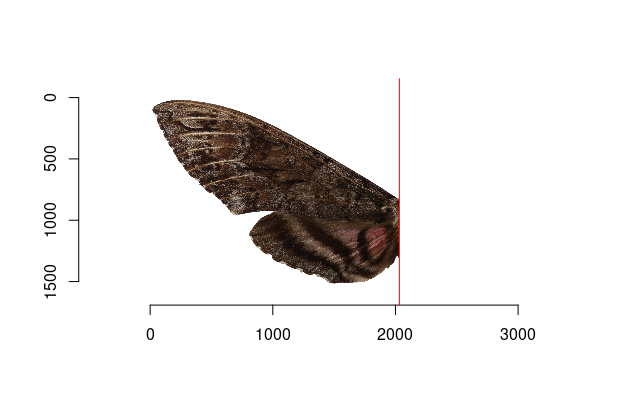
\includegraphics[width=\textwidth,height=2.08333in]{./img/Moment_of_inertia_about_the_axis.png}

\hypertarget{geometric-classification-and-measurement-of-wing-parameters}{%
\subsection{Geometric classification and measurement of wing
parameters}\label{geometric-classification-and-measurement-of-wing-parameters}}

In order to highlight the characteristic features of the butterfly
wings, it is of interest to approximate the butterfly wing using
polygons{[}\protect\hyperlink{ref-Bronstein2008}{3}{]}. A simplified
representation of a wings shape allows you to highlight the main
geometric properties.

\hypertarget{left-wing-of-hemaris-diffinis}{%
\subsubsection{Left wing of Hemaris
diffinis}\label{left-wing-of-hemaris-diffinis}}

\begin{figure}
\centering
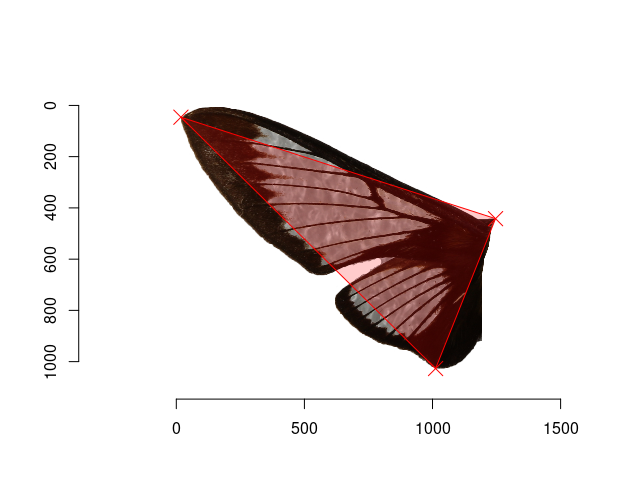
\includegraphics[width=\textwidth,height=3.125in]{./img/Areas_3_Hemaris_diffinis_left_wing.png}
\caption{Threangle}
\end{figure}

\begin{figure}
\centering
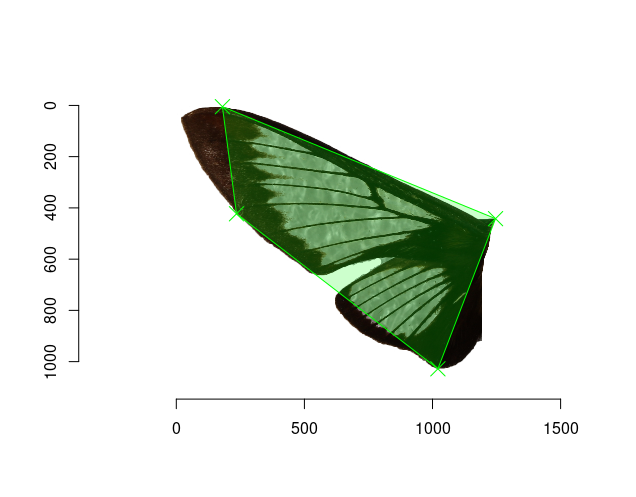
\includegraphics[width=\textwidth,height=3.125in]{./img/Areas_4_Hemaris_diffinis_left_wing.png}
\caption{Quadrangle}
\end{figure}

\begin{figure}
\centering
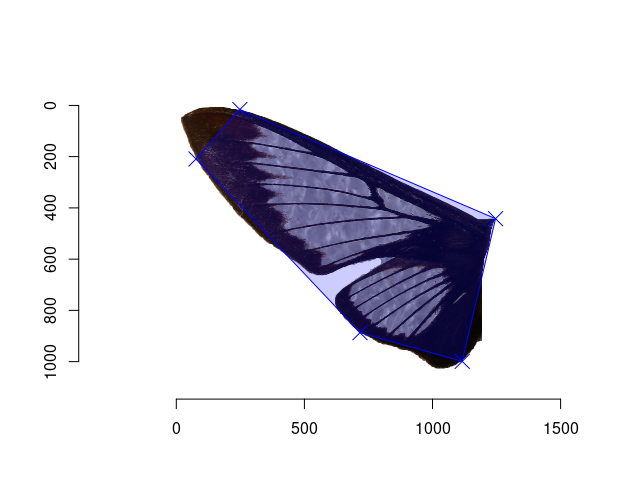
\includegraphics[width=\textwidth,height=3.125in]{./img/Areas_5_Hemaris_diffinis_left_wing.png}
\caption{Pentagon}
\end{figure}

\begin{figure}
\centering
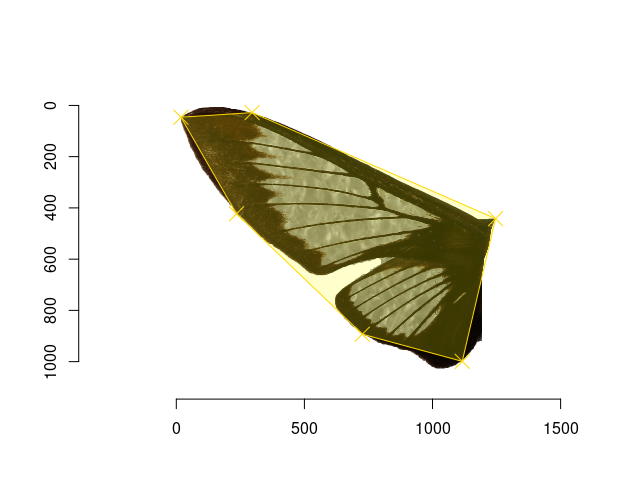
\includegraphics[width=\textwidth,height=3.125in]{./img/Areas_6_Hemaris_diffinis_left_wing.png}
\caption{Hexagon}
\end{figure}

\begin{figure}
\centering
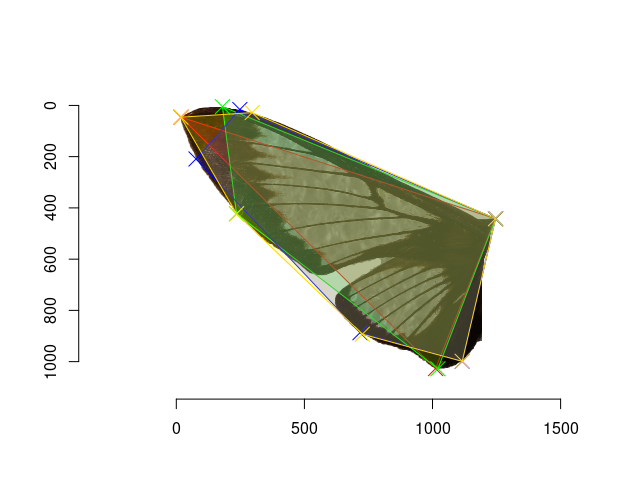
\includegraphics[width=\textwidth,height=3.125in]{./img/Areas_3_4_5_6_Hemaris_diffinis_left_wing.png}
\caption{Superposition of polygons}
\end{figure}

\hypertarget{left-wing-of-manduca-rustica}{%
\subsubsection{Left wing of Manduca
rustica}\label{left-wing-of-manduca-rustica}}

\begin{figure}
\centering
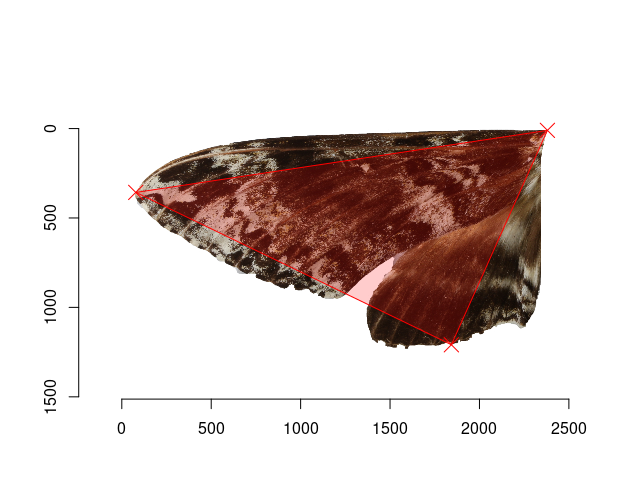
\includegraphics[width=\textwidth,height=3.125in]{./img/Areas_3_Manduca_rustica_left_wing.png}
\caption{Threangle}
\end{figure}

\begin{figure}
\centering
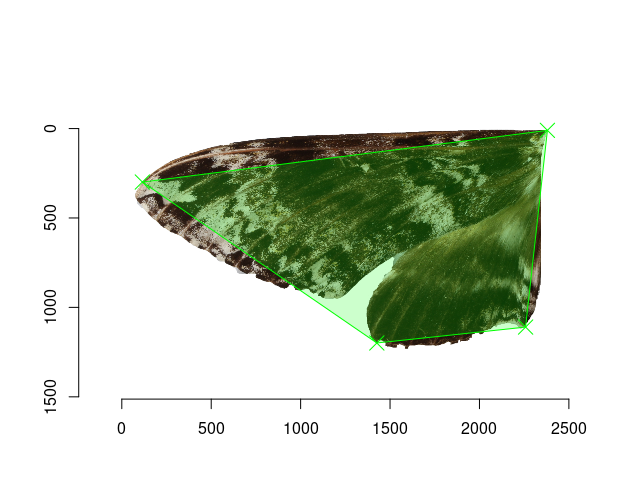
\includegraphics[width=\textwidth,height=3.125in]{./img/Areas_4_Manduca_rustica_left_wing.png}
\caption{Quadrangle}
\end{figure}

\begin{figure}
\centering
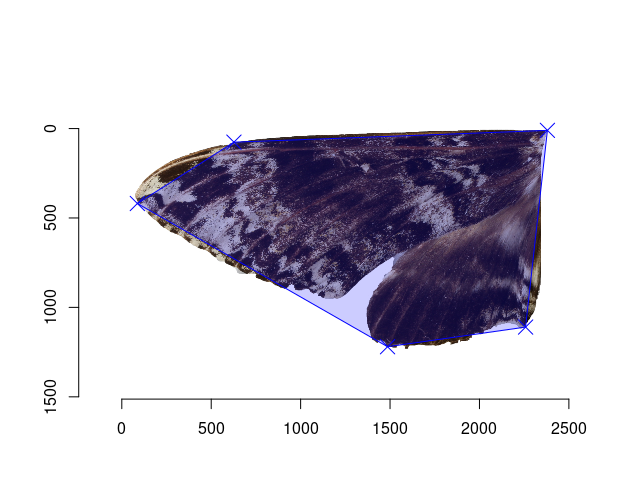
\includegraphics[width=\textwidth,height=3.125in]{./img/Areas_5_Manduca_rustica_left_wing.png}
\caption{Pentagon}
\end{figure}

\begin{figure}
\centering
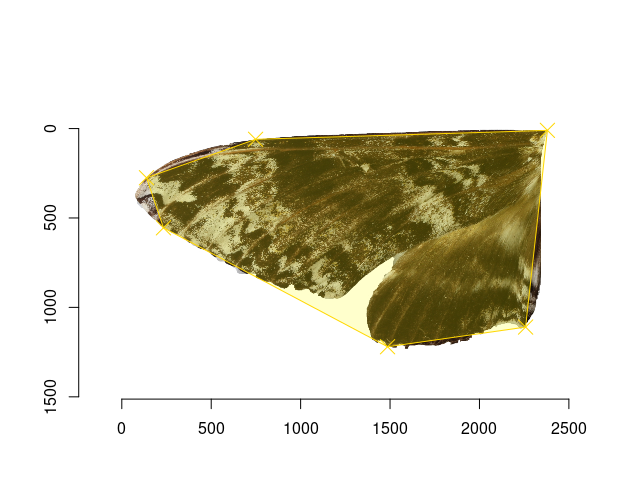
\includegraphics[width=\textwidth,height=3.125in]{./img/Areas_6_Manduca_rustica_left_wing.png}
\caption{Hexagon}
\end{figure}

\begin{figure}
\centering
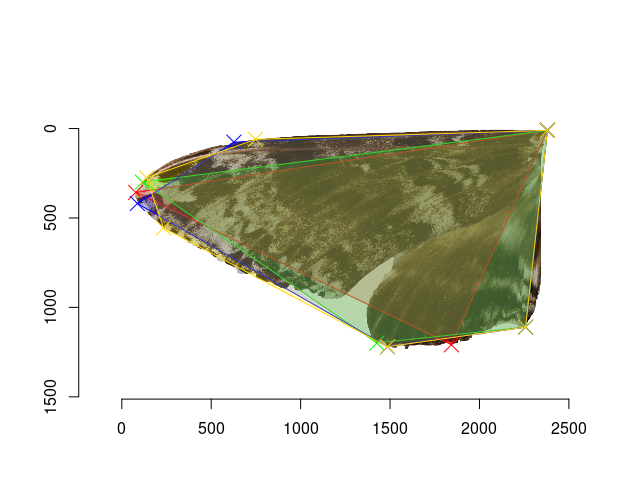
\includegraphics[width=\textwidth,height=3.125in]{./img/Areas_3_4_5_6_Manduca_rustica_left_wing.png}
\caption{Superposition of polygons}
\end{figure}

\hypertarget{butterfly-wing-boundary-definition}{%
\subsubsection{Butterfly wing boundary
definition}\label{butterfly-wing-boundary-definition}}

To find the boundaries of objects in images, one of the most common
algorithms is the Canny algorithm
{[}\protect\hyperlink{ref-Canny-edge}{4}{]}.

\begin{figure}
\centering
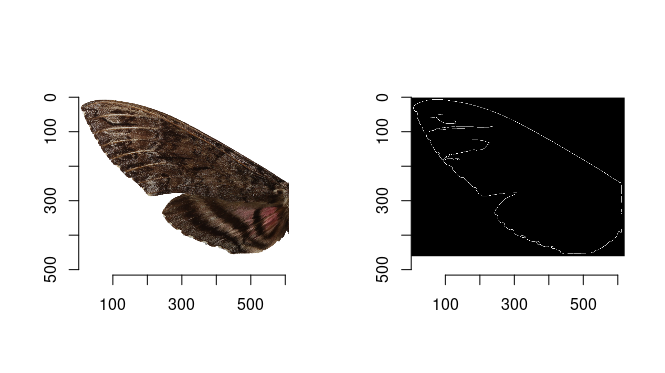
\includegraphics[width=7.29167in,height=\textheight]{./img/Canny_edge_0.png}
\caption{Finding edges in a color image}
\end{figure}

When using this algorithm, the boundaries will be found not only outside
the object but also inside. To avoid this, we can first convert the
image to black and white. The disadvantage of using this algorithm is
that at the output we have an unordered point cloud, which is the edge
of the object.

\begin{figure}
\centering
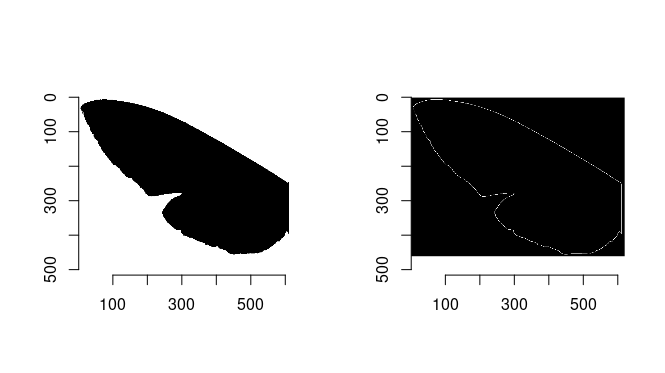
\includegraphics[width=\textwidth,height=7.29167in]{./img/Canny_edge_1.png}
\caption{Finding edges in a contrasting black and white image}
\end{figure}

The boundary of the butterfly wing object is actually a concave hull.
One of the algorithms for finding the edges of a concave hull is the
Alpha shape algorithm {[}\protect\hyperlink{ref-Alpha-shape}{5}{]}.

\begin{figure}
\centering
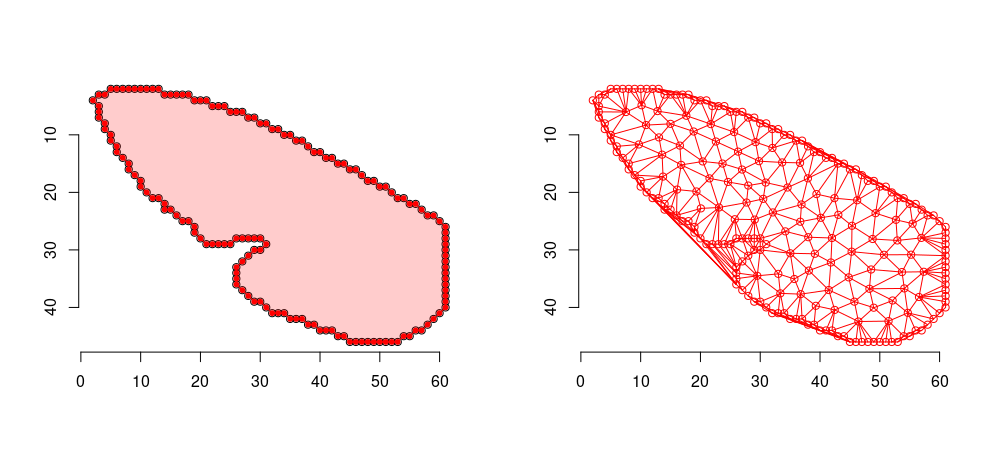
\includegraphics[width=\textwidth,height=7.29167in]{./img/Alpha_shape_0.png}
\caption{Concave Hull of a wing object}
\end{figure}

As a result of the Alpha shape algorithm, we can get a polygon that does
not intersect itself and has no holes. To find the area of such polygon,
we can use the shoelace Gauss algorithm.
{[}\protect\hyperlink{ref-Shoelace-formula}{6}{]}

\begin{figure}
\centering
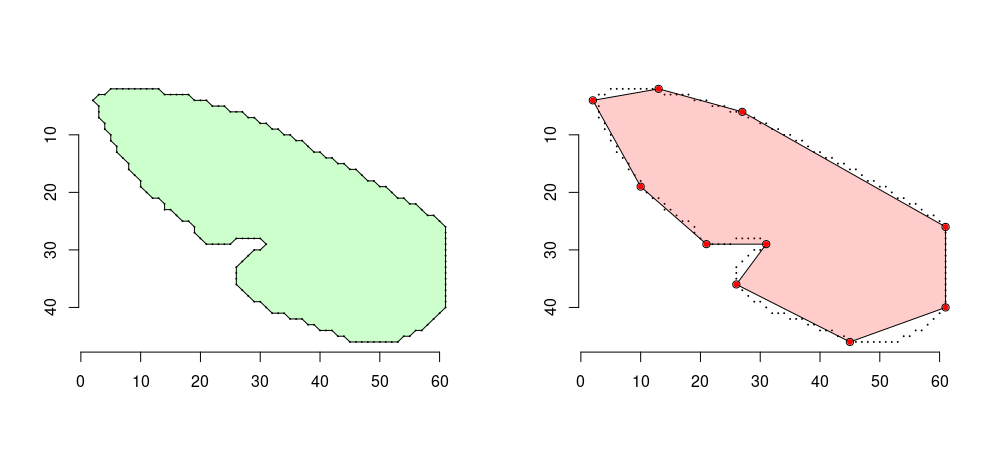
\includegraphics[width=\textwidth,height=7.29167in]{./img/Alpha_shape_1.png}
\caption{Concave hull after minimizing the number of points}
\end{figure}

\hypertarget{to-be-continued}{%
\subsection{To be continued\ldots{}}\label{to-be-continued}}

\begin{figure}
\centering
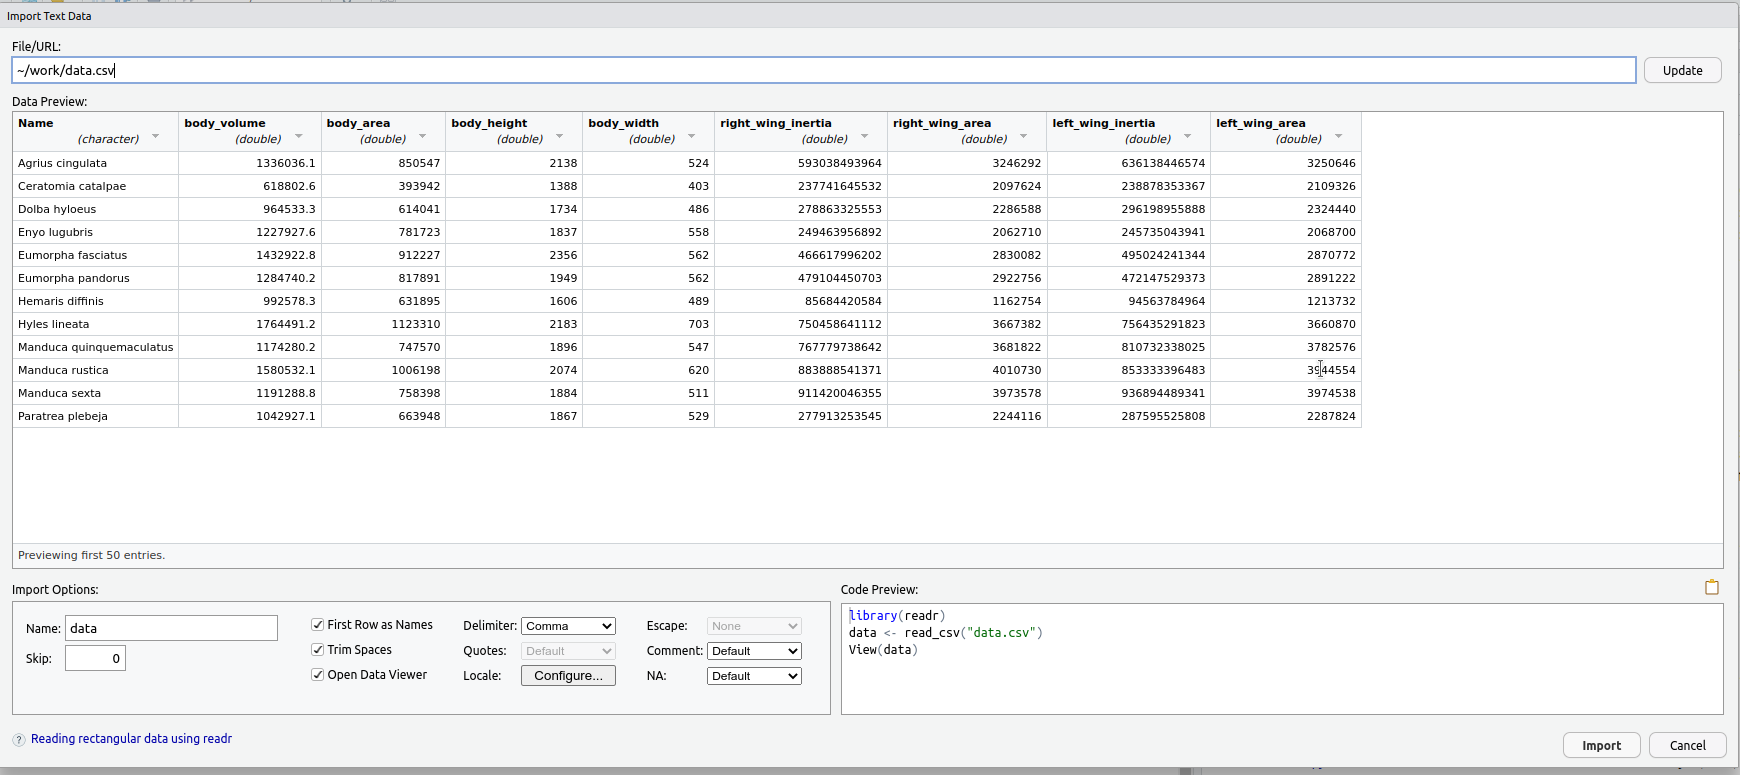
\includegraphics[width=\textwidth,height=4.16667in]{./img/data.png}
\caption{At the moment, the results of the calculations look like this}
\end{figure}

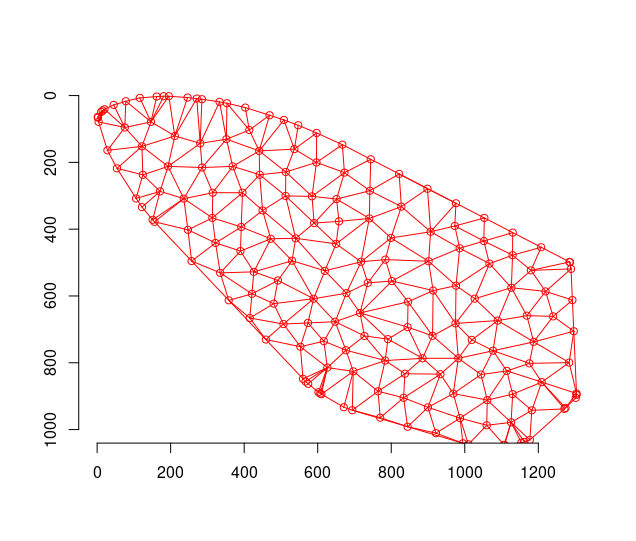
\includegraphics[width=\textwidth,height=2.60417in]{./img/convex_triangles.png}
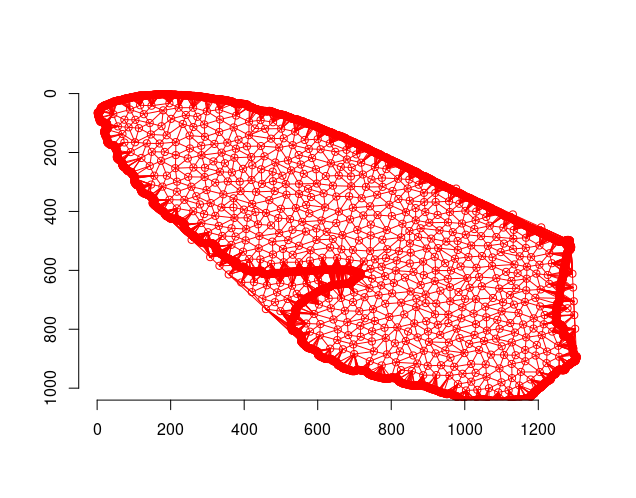
\includegraphics[width=\textwidth,height=2.60417in]{./img/edge_triangles.png}

\hypertarget{references}{%
\section{References}\label{references}}

\hypertarget{refs}{}
\begin{CSLReferences}{0}{0}
\leavevmode\vadjust pre{\hypertarget{ref-R-base}{}}%
\CSLLeftMargin{1. }
\CSLRightInline{R Core Team (2022) \href{https://www.R-project.org}{R: A
language and environment for statistical computing}, Vienna, Austria, R
Foundation for Statistical Computing.}

\leavevmode\vadjust pre{\hypertarget{ref-Insect-flight}{}}%
\CSLLeftMargin{2. }
\CSLRightInline{Wikipedia.org (2022)
\href{https://en.wikipedia.org/wiki/Insect_flight\#Indirect_flight}{Insect
indirect flight}.}

\leavevmode\vadjust pre{\hypertarget{ref-Bronstein2008}{}}%
\CSLLeftMargin{3. }
\CSLRightInline{Bronstein EM (2008)
\href{https://doi.org/10.1007/s10958-008-9144-x}{Approximation of convex
sets by polytopes}. \emph{J Math Sci} 153: pages727--762.}

\leavevmode\vadjust pre{\hypertarget{ref-Canny-edge}{}}%
\CSLLeftMargin{4. }
\CSLRightInline{Wikipedia.org (2022)
\href{https://en.wikipedia.org/wiki/Canny_edge_detector}{Canny edge
detector}.}

\leavevmode\vadjust pre{\hypertarget{ref-Alpha-shape}{}}%
\CSLLeftMargin{5. }
\CSLRightInline{Wikipedia.org (2022)
\href{https://en.wikipedia.org/wiki/Alpha_shape}{Alpha shape}.}

\leavevmode\vadjust pre{\hypertarget{ref-Shoelace-formula}{}}%
\CSLLeftMargin{6. }
\CSLRightInline{Wikipedia.org (2022)
\href{https://en.wikipedia.org/wiki/Shoelace_formula}{Gauss's area
formula}.}

\end{CSLReferences}

\end{document}
